\documentclass[12pt]{beamer}
\usetheme{Warsaw} 
% Warsaw, CambridgeUS
%\usecolortheme{Beaver}
%\usecolortheme{Wolverine}
\usepackage[utf8]{inputenc}
\usepackage{amsmath}
\usepackage{amsfonts}
\usepackage{amssymb}
\usepackage{graphicx}
\usepackage{xcolor}

\title{Presentation in Beamer}
\subtitle{How to build a Presentation}
\author{Nicolas Peter Lane}
\institute{Universidade Estadual de Santa Catarina}
\date{\today}

\begin{document}

\begin{frame}[shrink]
\titlepage
\end{frame}

\begin{frame}
\frametitle{Table of Contents}
\tableofcontents
\end{frame}

\section{Section 1}
\subsection{SS 1}
\begin{frame}[shrink]
\frametitle{Frame 1}
\begin{block}{Frame 1}
\pause
Contents of Frame 1

Lists example
\begin{itemize}
\item{A}
\begin{itemize}
\item{A.1}
\item{A.2}
\end{itemize}
\item{B}
\begin{itemize}
\item{B.1}
\item{B.2}
\end{itemize}
\end{itemize}

\end{block}
\end{frame}

\subsection{SS 2}
\begin{frame}[shrink]
\frametitle{Frame 2}
\begin{block}{Frame 2}
\pause
Contents of Frame 2

Enumeration example
\begin{enumerate}
\item{A}
\begin{enumerate}
\item{A.1}
\item{A.2}
\end{enumerate}
\item{B}
\begin{enumerate}
\item{B.1}
\item{B.2}
\end{enumerate}
\end{enumerate}

\end{block}
\end{frame}

\section{Section 2}
\subsection{SS 3}
\begin{frame}[shrink]
\frametitle{Frame 3}
\begin{block}{Frame 3}
\pause
Contents of Frame 3

Enumeration example
\begin{enumerate}[I]
\item{A}
\begin{enumerate}[i]
\item{A.1}
\item{A.2}
\end{enumerate}
\item{B}
\begin{enumerate}[(i)]
\item{B.1}
\item{B.2}
\end{enumerate}
\end{enumerate}

\end{block}
\end{frame}

\subsection{SS 4}
\begin{frame}[shrink]
\frametitle{Frame 4}
\begin{block}{Frame 4}
\pause
Contents of Frame 4

Enumeration example
\begin{enumerate}[I]
\item{A}
\begin{itemize}
\item{A.1}
\item{A.2}
\end{itemize}
\item{B}
\begin{enumerate}[(i)]
\item{B.1}
\item{B.2}
\end{enumerate}
\end{enumerate}

\end{block}
\end{frame}

\section{Section 3}
\subsection{SS 5}
\begin{frame}[shrink]
\frametitle{Frame 5}
\begin{block}{Frame 5}
\pause
Contents of Frame 5

\begin{itemize}
\item{Images}

\begin{figure}
\centering
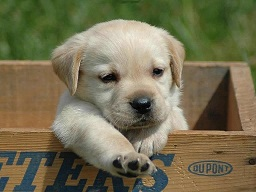
\includegraphics[height=2cm, width=3cm]{dog}
\caption{A dog}
\end{figure}

\end{itemize}
\end{block}
\end{frame}

\begin{frame}[shrink]
\frametitle{Frame 6}
\begin{block}{Frame 6}
\pause
Contents of Frame 6

Columns example

\begin{columns}
\column{0.5\textwidth}
Aaaaaaaaaaaa aaaaaaaaaaaaaaaaaaa aaaaaaaaaaaaaaaaaaaaaa
Aaaaaaaaaaaa aaaaaaaaaaaaaaaaaaa aaaaaaaaaaaaaaaaaaaaaa
Aaaaaaaaaaaa aaaaaaaaaaaaaaaaaaa aaaaaaaaaaaaaaaaaaaaaa
Aaaaaaaaaaaa aaaaaaaaaaaaaaaaaaa aaaaaaaaaaaaaaaaaaaaaa

\column{0.5\textwidth}
\begin{figure}
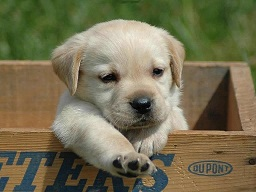
\includegraphics[height=3cm, width=4cm]{dog}
\caption{A dog}
\end{figure}

\end{columns}
\end{block}
\end{frame}

\begin{frame}[shrink]
\frametitle{Frame 7}
\begin{block}{Frame 7}
\pause
Contents of Frame 7

Description example

\begin{description}
\item[API] Application Programming Interface
\item[LAN] Local Area Interface
\item[ASCII] Americam Standart Code for Information Schange
\end{description}
\end{block}
\end{frame}

\begin{frame}[shrink]
\frametitle{Frame 7}
\begin{block}{Frame 7}
\pause
Contents of Frame 7

Table example

\begin{table}
\begin{tabular}{c|c|c|c|c|c}
O & O & O & O & O\\
\hline \hline
A & B & C & D & E \\
F & G & H & I & J \\
K & L & M & D & N \\
\end{tabular}
\caption{Table example}
\end{table}

\end{block}
\end{frame}

\end{document}
